\section{Durchführung}
\label{sec:Durchführung}

\begin{figure}
    \centering
    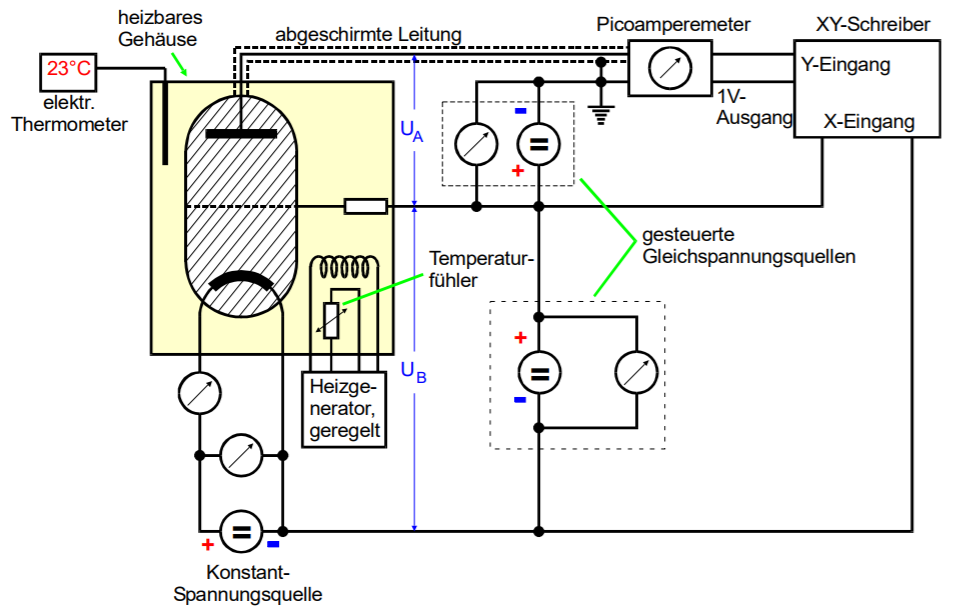
\includegraphics[width=\textwidth]{content/schaltskizze.PNG}
    \caption{Schaltskizze des Versuches\cite{V601}.}
    \label{fig:schaltskizze}
\end{figure}

Zunächst wird die Schaltung gemäß der Skizze in \autoref{fig:schaltskizze} aufgebaut. 
Dabei ist zu beachten, dass an dem Schreiber nicht immer $U_\text{B}$ anliegt, sondern jeweils die zu messende Spannung.
Der Schreiber wird mittels der "Zero"-Drehknöpfen so kalibriert, dass sich der Nullpunkt in der unteren linken Ecke befindet. 
Des Weiteren ist vor jeder Messung darauf zu achten, dass der Schreiber so skaliert ist, 
dass er nie über seinen Maximalausschlag hinaus geht, um Datenverlust zu verhindern.

Zunächst wird Bremsspannung $U_\text{A}$ untersucht, um die integrale Energieverteilung der Elektronen zu untersuchen.
Die Beschleunigungsspannung $U_\text{B}$ wird auf konstant $+11$ V eingestellt. 
Zunächst wird eine Messung des Auffängerstroms $I_\text{A}$ bei Zimmertemperatur durchgeführt und anschließend weitere Messungen bei $140 - 160$ °C.
Nun wird die die Bremsspannung von 0 V bis auf ihren Maximalwert langsam variiert. 
Die dadurch entstehende Kurve von $I_\text{A}$ in Abhängigkeit von $U_\text{A}$ wird durch den Schreiber notiert.

Als nächstes werden Franck-Hertz-Kurven bei verschiedenen Temperaturen zwischen $160 \text{°C} \leq T \leq 200 \text{°C}$ aufgenommen. 
Dazu wird die Schaltung nun so aufgebaut, dass $U_\text{B}$ am Schreiber anliegt.
Die Bremsspannung wird dabei auf $U_\text{A} = -1$ V eingestellt. 
Die Beschleunigungsspannung $U_\text{B}$ wird so variiert, dass sie zwischen 0 V und 60 V liegt.

Zuletzt wird die Spannung $U_\text{B}$ bestimmt, ab der Quecksilber ionisiert wird.
 Dazu wird die Temperatur zwischen $100$ und $110$ °C gehalten. Die Gegenspannung wird auf $U_\text{A} = 30$ V eingestellt.
Nun wird die Beschleunigungsspannung langsam erhöht, bis die Stromstärke $I_A$ beginnt rapide anzusteigen.